\documentclass{article}

\usepackage{graphicx}
\usepackage{tikz}
\usepackage{tikzsymbols}
\usetikzlibrary{calc,patterns,shapes.geometric}
\pagestyle{empty}
\usepackage[margin=0pt]{geometry}
\geometry{papersize={14in,12in}}

\def\centerarc[#1](#2)(#3:#4:#5){\draw[#1] ($(#2)+({#5*cos(#3)},{#5*sin(#3)})$) arc (#3:#4:#5);}

\begin{document}
	\begin{figure}
		\centering
		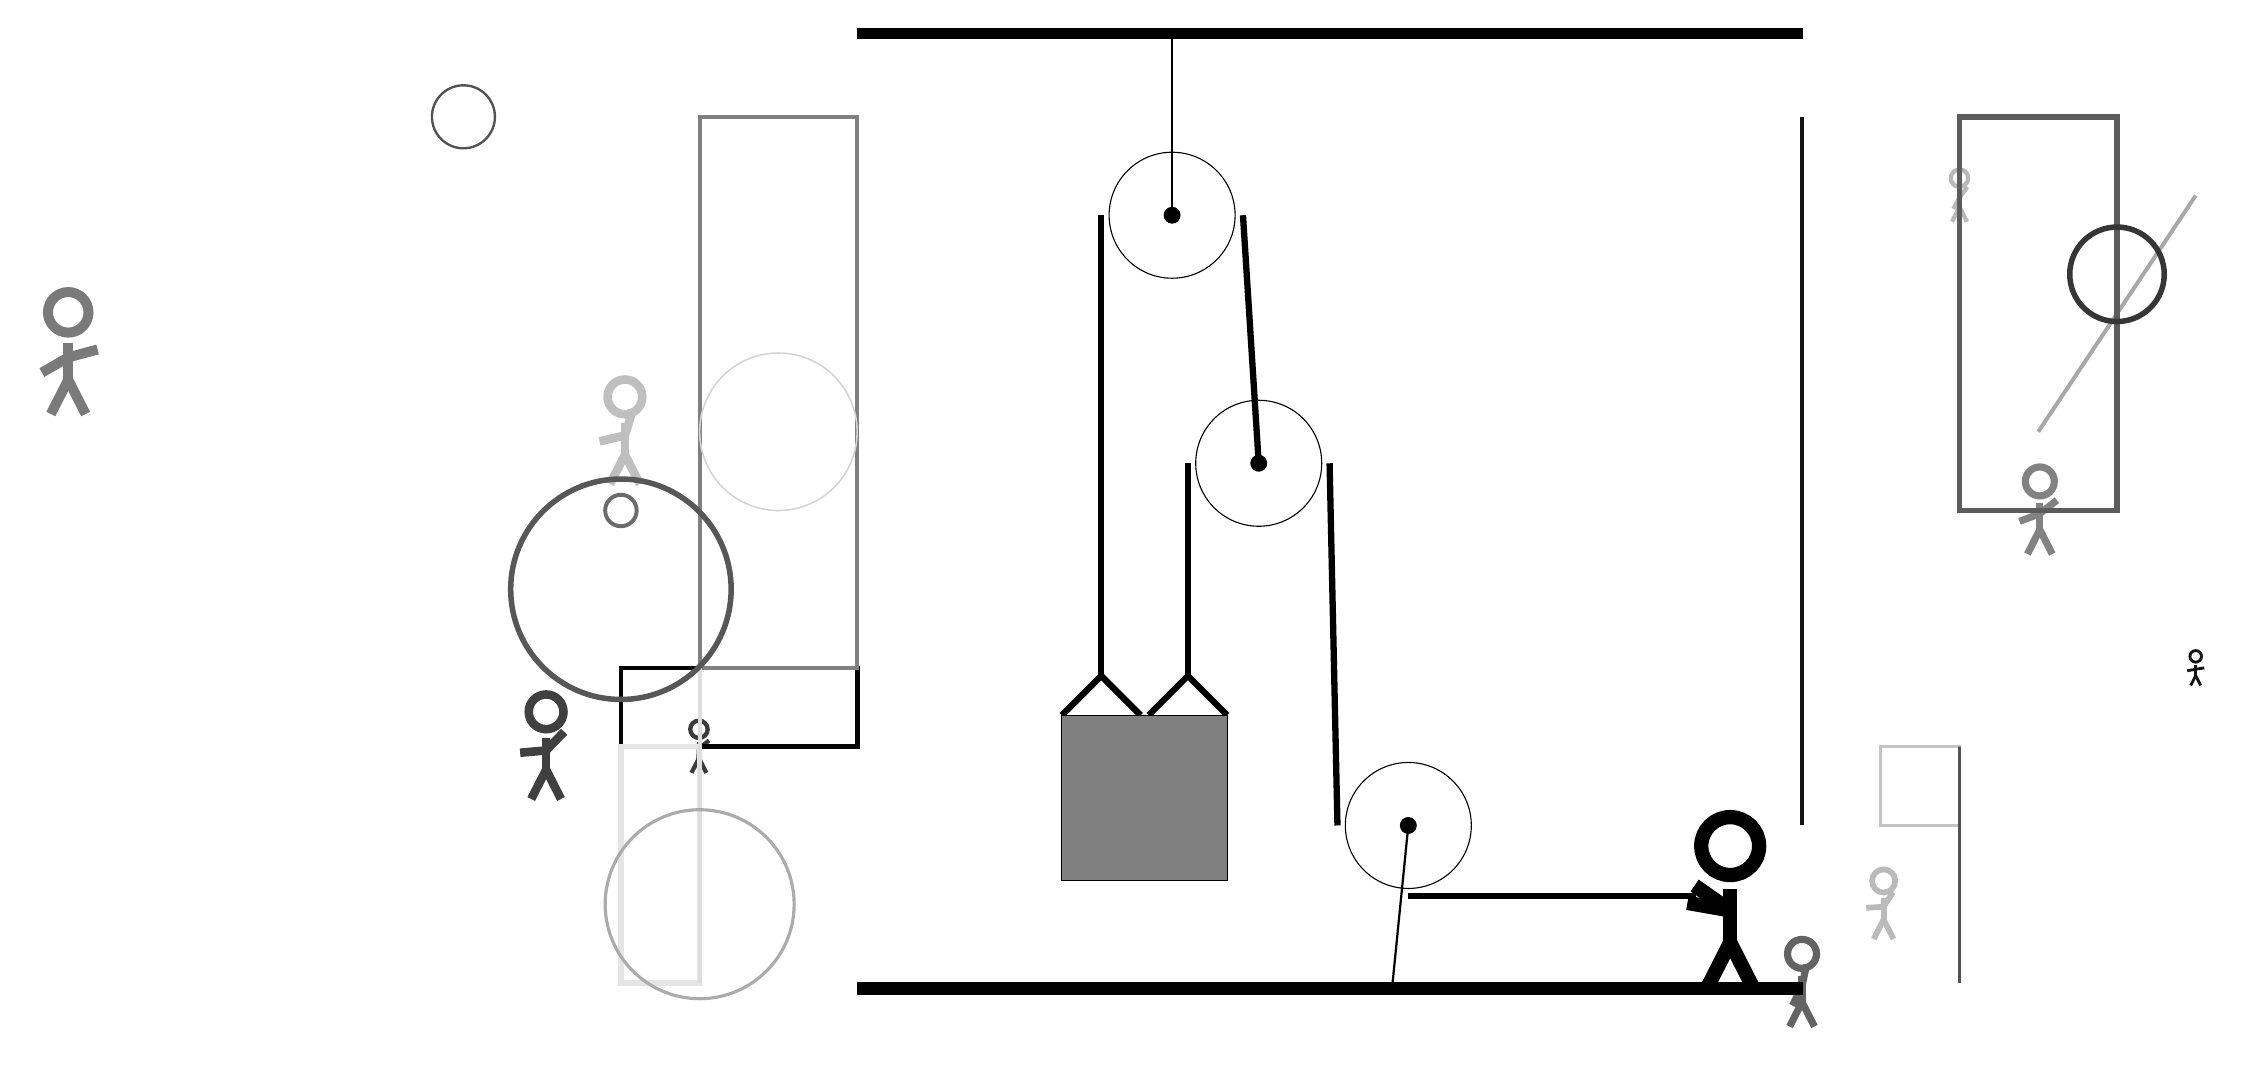
\begin{tikzpicture}
			%%%%% START %%%%%
			
			\draw[fill=black] (-2, 9) rectangle (10, 9.125);
			
			\draw (2, 6.75) circle (0.8);
			\draw[fill=black] (2, 6.75) circle (0.1);
			\draw[thick] (2, 6.75) -- (2, 9);
			
			\draw (3.1, 3.6) circle (0.8);
			\draw[fill=black] (3.1, 3.6) circle (0.1);
			
			\draw (5, -1) circle (0.8);
			\draw[fill=black] (5, -1) circle (0.1);
			\draw[thick] (5, -1) -- (4.8, -3);
			
			\draw[line width = 0.8mm]  (0.6, 0.4) -- (1.1, 0.9) -- (1.6, 0.4);
			\draw[line width = 0.8mm]  (1.7, 0.4) -- (2.2, 0.9) -- (2.7, 0.4);
			\draw[fill=black!50] (0.6, 0.4) rectangle (2.7, -1.7);
			
			\draw[line width = 0.8mm] (1.1, 6.75) -- (1.1, 0.9);
			\centerarc[line width = 0.8mm](2, 6.75)(0:180:0.9);
			\draw[line width = 0.8mm] (2.9, 6.75) -- (3.1, 3.6);
			\draw[line width = 0.8mm] (2.2, 3.6) -- (2.2, 0.9);
			\centerarc[line width = 0.8mm](3.1, 3.6)(0:180:0.9);
			\draw[line width = 0.8mm] (4.0, 3.6) -- (4.1, -1);
			\centerarc[line width = 0.8mm](5, -1)(180:270:0.9);
			\draw[line width = 0.8mm] (5, -1.9) -- (8.65, -1.9);
			
			\node at (9, -2) {\Strichmaxerl[10][-35][170]};
			
			\node[line width=0.6mm, color=black!25] at (-5, 4) {\Strichmaxerl[6][13][73]};
			
			\draw[line width=0.4mm, color=black!23] (12, 0) rectangle (11, -1);
			\node[line width=0.4mm, color=black!28] at (12, 7) {\Strichmaxerl[3][62][53]};
			\draw [line width=0.5mm, color=black!58](-5, 3) circle (0.2);
			\node[line width=0.7mm, color=black!52] at (-12, 5) {\Strichmaxerl[7][30][15]};
			
			\draw[line width=0.5mm, color=black!34](13, 4) -- (15, 7);
			
			\draw [line width=0.3mm, color=black!68](-7, 8) circle (0.4);
			\node[line width=0.7mm, color=black!49] at (13, 3) {\Strichmaxerl[5][21][38]};
			\draw[line width=0.5mm, color=black!92](10, 8) -- (10, -1);
			
			\node[line width=0.5mm, color=black!77] at (-4, 0) {\Strichmaxerl[3][87][39]};
			\node[line width=0.7mm, color=black!92] at (15, 1) {\Strichmaxerl[2][10][9]};
			\draw[line width=0.6mm, color=black!98] (-2, 1) rectangle (-5, 0);
			\draw[line width=0.7mm, color=black!64] (12, 8) rectangle (14, 3);
			\draw[line width=0.7mm, color=black!10] (-4, 0) rectangle (-5, -3);
			\draw[line width=0.5mm, color=black!50] (-2, 8) rectangle (-4, 1);
			\draw [line width=0.2mm, color=black!17](-3, 4) circle (1.0);
			\draw[line width=0.3mm, color=black!68] (12, -3) rectangle (12, 0);
			
			\draw[line width=0.5mm, color=black!13](-4, -3) -- (-4, 1);
			\draw [line width=0.7mm, color=black!79](14, 6) circle (0.6);
			\draw [line width=0.7mm, color=black!66](-5, 2) circle (1.4);
			\draw [line width=0.4mm, color=black!33](-4, -2) circle (1.2);
			\node[line width=0.3mm, color=black!27] at (11, -2) {\Strichmaxerl[4][4][57]};
			\node[line width=0.3mm, color=black!61] at (10, -3) {\Strichmaxerl[5][64][78]};
			\node[line width=0.6mm, color=black!75] at (-6, 0) {\Strichmaxerl[6][5][46]};
			
			\draw[fill=black] (-2, -3) rectangle (10, -3.15);
			
			%%%%% END %%%%%
		\end{tikzpicture}
	\end{figure}	
\end{document}